\documentclass[12pt]{article}
\usepackage{indentfirst, mathtools, amsfonts, amsthm, graphicx, multicol}

\usepackage{tikz}
\usetikzlibrary{arrows,positioning, calc,trees}

\tikzstyle{vertex}=[draw,fill=black!15,rectangle,minimum size=20pt,inner sep=0pt]

\newtheorem{theorem}{Theorem}[section]
\newtheorem{corollary}[theorem]{Corollary}
\newtheorem{lemma}[theorem]{Lemma}

\theoremstyle{definition}
\newtheorem{definition}[theorem]{Definition}


\title{CSC 544 Project Report}
\author{Richard Spence}
\date{December 6, 2017}

\begin{document}
\maketitle

\section{Introduction}
This project investigates an edge-constrained variant of the Euclidean $t$-spanner. $t$-spanners have applications in network planning and telecommunications; however, they can be useful in visualizing relationships between various fields. For example, our RWG under TRIPODS is looking at a multi-level variant of the $t$-spanner problem as a way to represent such relationships.

\section{Preliminaries}
$t$-spanners can be defined for arbitrary weighted graphs; however we will focus on Euclidean $t$-spanners.

\begin{definition}
Given a set $V$ of points in $\mathbb{R}^2$ and a real number $t \ge 1$, a \emph{t-spanner} over $V$ is an undirected graph $G = (V, E)$ consisting of straight-line edges such that the following hold:

\begin{itemize}
\item $G$ spans all points in $V$.
\item For all $u, v \in V$, we have $\delta_{G}(u,v) \le t \cdot d(u,v)$ where $\delta_G(u,v)$ denotes the length of the shortest path from $u$ to $v$ in $G$, and $d(u,v)$ denotes the Euclidean distance from $u$ to $v$.
\end{itemize}
\end{definition}

The constant $t$ is called the \emph{stretch factor}, and the each edge in $G$ has weight equal to its distance. The $t$-spanner problem is to find a Euclidean $t$-spanner of minimum total length; however, this problem is NP-hard for all $t > 1$ \cite{Carmi}.

%talk about t-spanners on arbitrary graphs

We introduce an edge-constrained variant of a Euclidean $t$-spanner, which we will denote a $(k,t)$-spanner.

\begin{definition}[$(k,t)$-spanner] Given a set $V$ of points in the plane, a real number $t \ge 1$, and an integer $k \ge 1$, we will define a \emph{$(k,t)$-spanner} over $V$ to be a $t$-spanner $G = (V,E)$ with the additional property that for all $u,v \in V$, there exists a path from $u$ to $v$ of length at most $t \cdot d(u,v)$ that uses no more than $k$ edges in $G$.
\end{definition}

If $k = |V|-1$, the above definition is equivalent to a Euclidean $t$-spanner. Every set $V$ has a $(k,t)$ spanner, since the complete graph $K_{|V|}$ is a $(1,1)$-spanner. A natural question is the $(k,t)$-spanner problem: given $V$, a real number $t \ge 1$, and an integer $k \ge 1$, return a $(k,t)$-spanner over $V$ with minimum total length. As this generalizes the Euclidean $t$-spanner problem, this is also NP-hard.

The main motivation behind the $(k,t)$-spanner problem is in route or flight planning. For example, an airline may wish to install flight routes in order to ensure passengers do not travel excessive distance nor make too many layovers to reach their destination, while at the same time, minimizing its cost. This problem could also be applied to visualization, particularly if one wishes to see how various fields are related; an example is in Figure \ref{fig:fields}.

\begin{figure}[h]
\begin{center}
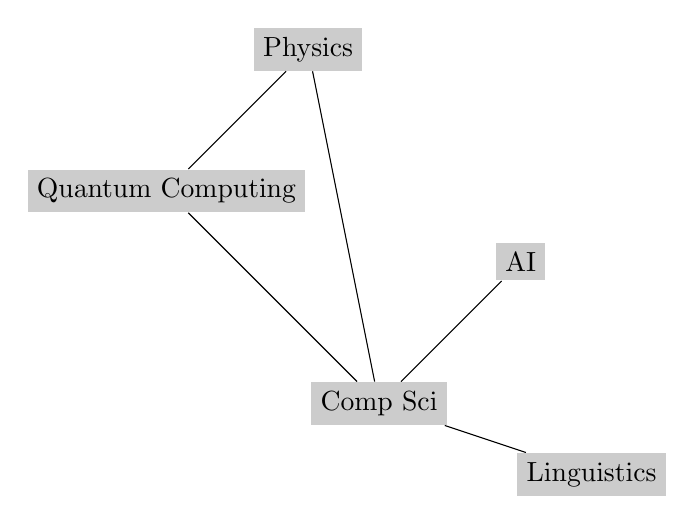
\begin{tikzpicture}
  [scale=.9,auto=left,every node/.style={rectangle,fill=black!20}]
  \node (n1) at (4,1) {Comp Sci};
  \node (n2) at (7,0) {Linguistics};
  \node (n3) at (6,3) {AI};
  \node (n4) at (3,6) {Physics};
  \node (n5) at (1,4) {Quantum Computing};

  \foreach \from/\to in {n1/n2, n1/n3, n1/n4, n1/n5, n4/n5}
    \draw (\from) -- (\to);
\end{tikzpicture}
\end{center}
\caption{Example $(2,t)$-spanner showing relationships between various fields.}
\label{fig:fields}
\end{figure}

\section{A Simple Heuristic}
The following greedy solution can be used to compute a $(k,t)$-spanner: start with the complete graph $K_{|V|}$, sort all $\binom{|V|}{2}$ edges in non-increasing order of distance. For each edge $e \in E$, determine whether the graph obtained by removing edge $e$ is a $(k,t)$-spanner, and if so, remove $e$.

\begin{verbatim}
//start with complete graph
E = {(i,j), 1 <= i,j <= n}
sort E in non-increasing order
for e in E:
   E' = E \ e
   if (V, E') is a (k,t)-spanner:
       E' = E
return E
\end{verbatim}

However, checking whether a dense graph is a $(k,t)$-spanner proved difficult to implement in terms of running time, since this could potentially take $|V|^k$ time checking all length-$k$ paths from some vertex $u$ (since shortest paths need not have at most $k$ edges). A breadth-first search (BFS) may not necessarily work since once a vertex is revisited, the algorithm stops exploring paths at that vertex.

A simpler heuristic (implemented in the project) that still produces a valid solution only removes an edge $e$ if for the resulting graph $G' = (V,E')$, the shortest path between any two vertices $u$ and $v$ is at most $t \cdot d(u,v)$, and comprises at most $k$ edges. Figures \ref{fig:example} and \ref{fig:hub} show examples on random sets of $|V| = 30$ points.

\begin{figure}[h]
\centering
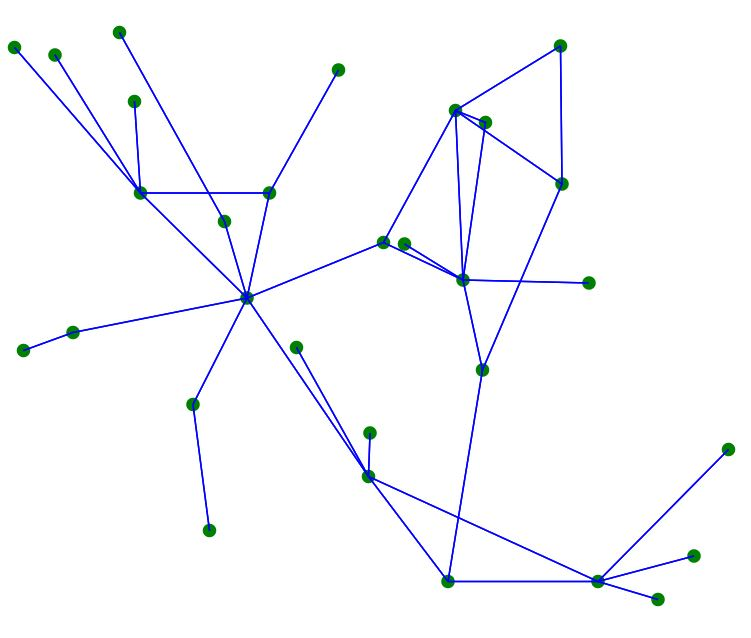
\includegraphics[width=3in]{images/spanner}
\caption{A $(5,10)$-spanner produced by running the heuristic on a random set of $|V| = 30$ vertices.}
\label{fig:example}
\end{figure}

\section{Approximation Bounds}
A suitable way to analyze performance is to compare with the minimum spanning tree (MST) over the same set of points. If $k = |V|-1$ and $t$ is arbitrarily large, the spanner solution is very close or equal to the MST, which is expected. The approximation ratio will likely depend on $k$, $t$, $|V|$, and the distance metric used, and no approximation ratios are known.

The case $k = 2$ might be an interesting problem, since it is easier to establish which edges \emph{must} be contained in a $(2,t)$-spanner. In particular, for any $u, v \in V$, there must be a path $u \to w \to v$ where $w$ is contained in the ellipse whose foci are $u$ and $v$, with major axis $t \cdot d(u,v)$. If no such $w$ exists, then $(u,v)$ must be an edge in any $(2,t)$-spanner. Additionally, for $k = 2$ and large $t$, the optimal solution tends to resemble a hub-and-spoke graph (see Figure \ref{fig:hub} for an example), which is commonly used in transit systems.

\begin{figure}[h]
\centering
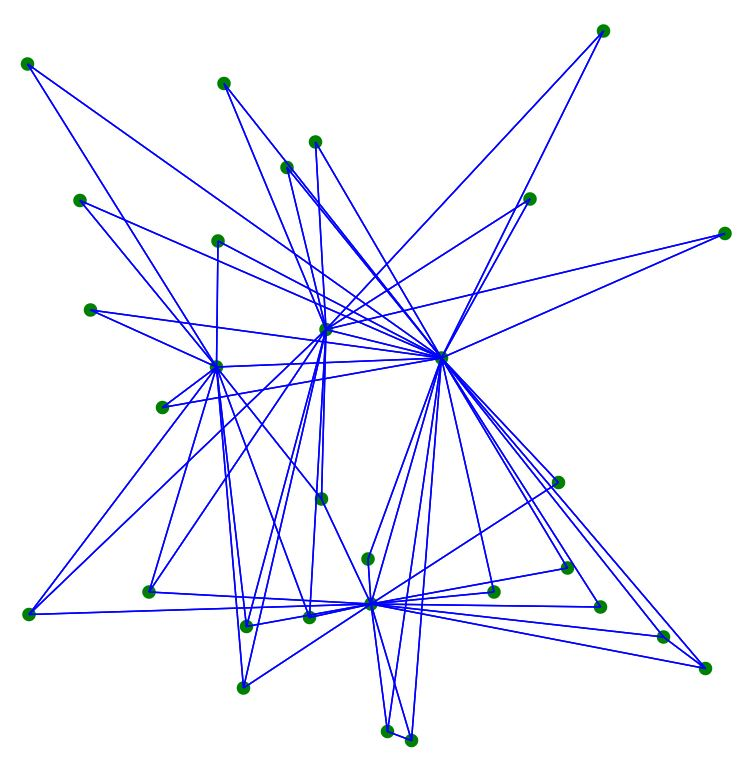
\includegraphics[width=3in]{images/spanner-2}
\caption{A $(2,10)$-spanner produced using the heuristic. Notice the formation of centralized ``hubs."}
\label{fig:hub}
\end{figure}

\section{Additional Questions}
There is literature on $t$-spanners, Euclidean $t$-spanners, and other variants of $t$-spanners, but I have not been able to find papers on this specific variant of the Euclidean $t$-spanner problem. Many interesting theoretical questions could be asked: Is the problem NP-hard for $k = 2$? What are the approximation ratios for the above heuristics? 

\newpage

 \bibliographystyle{ieeetr}
\bibliography{references}{}
\end{document}